\documentclass[a4paper,10pt,twoside]{article}
%\usepackage{amssymb}
%\usepackage{amsthm}
\usepackage[polish]{babel}
\usepackage[utf8]{inputenc}
\usepackage[T1]{fontenc}
\usepackage{indentfirst}
\usepackage{caption}
\usepackage[top=2.5cm, bottom=2.5cm, left=2.5cm, right=2.5cm]{geometry}
\usepackage{graphicx}
\usepackage{makecell}
\usepackage{amsmath}
\usepackage{booktabs}
\usepackage{multirow}


\begin{document}
	
	\begin{center}
		\bgroup
		\def\arraystretch{1.5}
		\begin{tabular}{|c|c|c|c|c|c|}
			\hline
			EAIiIB & \multicolumn{2}{|c|}{Michał Kilian} & Rok II & \multicolumn{2}{|c|}{Grupa 5a} \\
			\hline
			\multicolumn{3}{|c|}{\begin{tabular}{c}Temat: \\ Wahadło proste \end{tabular}} & 
			\multicolumn{3}{|c|}{\begin{tabular}{c}Numer ćwiczenia: \\ 0 \end{tabular}} \\
			\hline
			\begin{tabular}{@{}c@{}}Data wykonania\\10.10.2018r.\end{tabular} & \begin{tabular}{@{}c@{}}Data oddania\\12.10.2018r.\end{tabular} & 
			\begin{tabular}{c}Zwrot do\\poprawki\\\phantom{data} \end{tabular} & \begin{tabular}{c}Data oddania\\\phantom{data}\end{tabular} &
			\begin{tabular}{@{}c@{}}Data zaliczenia\\\phantom{data}\end{tabular} & \begin{tabular}{c}Ocena\\\phantom{ocena}\end{tabular} \\[4ex]
			\hline
		\end{tabular}
		\egroup
	\end{center}
	
	\section{Cel ćwiczenia}
	Zaznajomienie się
	z typowymi metodami opracowania danych pomiarowych
	przy wykorzystaniu wyników pomiarów dla wahadła pro
	stego 
	

	Wahadło matematyczne to punktowa masa $m$ zawieszona na nieważkiej i nierozciągliwej lince poruszająca w jednorodnym polu grawitacyjnym.
	W doświadczeniu wykorzystamy bardzo dobre przybliżenie takiego układu jakim jest ciężka metalowa kulka zawieszona na nitce.
	
	Aby znacząco uprościć obliczenia przyjmiemy $\sin\theta\approx\theta$ co jest prawdą dla małych wartości kąta $\theta$ zgodnie z
	twierdzeniem Taylora. Dzięki temu ograniczamy wpływ oporu powietza na wyniki, a z uproszczonego równania ruchu wahadła
	uzyskujemy następujacą zależność
	\begin{equation}
	T=2\pi\sqrt{\frac{l}{g}}
	\end{equation}
	gdzie $T$ - okres drgań, $l$ - długość nici, $g$ - przyspieszenie grawitacyjne. Po przekształceniu otrzymujemy wzór roboczy pozwalający
	na wyznaczenie wartości przyspieszenia grawitacyjnego dla Ziemi
	\begin{equation}
	\label{eq:working_g}
	g=\frac{4\pi^2l}{T^2}
	\end{equation}
	\newpage
	\section{Wykonanie ćwiczenia}
	
	\begin{enumerate}
		\item Zapoznać się z budową mikroskopu
		\item Na obu powierzchniach płytki zrobić kreski, jedna nad drugą cienkim pisakiem (ewentualnie wykorzystać istniejące kreski)
		\item Zmierzyć śrubą
		mikrometryczną
		grubość płytki d w pobliżu kresek. 
		\item Ustaw  badaną
		płytkę
		na  stoliku  mikroskopu  w  uchwycie  i  dobierz  ostrość
		tak  by  uzyskać
		kontrastowy obraz. Regulując położenie stolika pokrętłem 7a zaobserwuj górny i dolny 
		ślad zaznaczony na płytce. 
		\item Pokrętłem 7b przesuń stolik mikroskopu do momentu uzyskania ostrego obrazu śladu na górnej powierzchni płytki.
		\item Odczytaj położenie $a_g$ wskazówki czujnika mikrometrycznego. 
		\item Przesuń stolik mikroskopu do położenia, w którym widoczny jest ślad na dolnej powierzchni płytki (pokrętłem 7b). 
		\item Ponownie odczytaj położenie $a_d$ wskazóWki czujnika.
		\item Odczyty zanotuj w tabeli 1, 2 lub 3.
	\end{enumerate}
	
	
	\section{Wyniki pomiarów}
	\paragraph{Obliczenie grubości rzeczywistej dla płytki szklanej} WSTAWIĆ OBLICZENIA
\\	\begin{table}[!htbp]
		\caption{\textbf{}}
		\centering
		\def\arraystretch{1.4}
		\begin{tabular}{|c|c|c|c|}
			\hline
			\multicolumn{4}{|l|}{\makecell{materiał: szkło\hspace{115pt} \\ grubość rzeczywista d = WSTAWIĆ[mm] \\ niepewność \hspace{55pt}$u(d) = 0,01$[mm]\hspace{20pt}}} 
			\\ \hline
			\multirow{2}{*}{lp.} & \multicolumn{2}{c|}{Wskazanie czujnika} & \makecell{grubość \\pozorna } \\
			\cline{2-4}
			  
			\multirow{2}{*}{} & $a_d$[mm] & $a_g$[mm] & $h = a_d - a_g$[mm] \\ \hline
			1 & 4,19 & 1,13 & 3,06 \\ \hline
			2 & 4,23 & 1,02 & 3,21 \\ \hline
			3 & 4,22 & 1,14 & 3,08\\ \hline
			4 & 4,21 & 1,15 & 3,06\\ \hline
			5 & 4,17 & 1,17 & 3,00\\ \hline
			6 & 4,16 & 1,19 & 2,97\\ \hline
			7 & 4,16 & 1,17 & 2,99\\ \hline
			8 & 4,21 & 1,15 & 3,06\\ \hline
			9 & 4,19 & 1,17 & 3,02\\ \hline
			10 & 4,19 & 1,19 & 3,00\\ \hline
		\end{tabular}
	\end{table}
\begin{center}
	średnia grubość pozorna \textit{h} - \\
	niepewność \textit{u(h)} -
\end{center}
		\newpage
		\paragraph{Obliczenie grubości rzeczywistej dla płytki pleksiglasowej} WSTAWIĆ OBLICZENIA
		\\	\begin{table}[!htbp]
			\caption{\textbf{}}
			\centering
			\def\arraystretch{1.4}
			\begin{tabular}{|c|c|c|c|}
				\hline
				\multicolumn{4}{|l|}{\makecell{materiał: pleksiglas\hspace{95pt} \\ grubość rzeczywista d = WSTAWIĆ[mm] \\ niepewność \hspace{55pt}$u(d) = 0,01$[mm]\hspace{20pt}}} 
				\\ \hline
				\multirow{2}{*}{lp.} & \multicolumn{2}{c|}{Wskazanie czujnika} & \makecell{grubość \\pozorna } \\
				\cline{2-4}
				
				\multirow{2}{*}{} & $a_d$[mm] & $a_g$[mm] & $h = a_d - a_g$[mm] \\ \hline
				1 & 4,39 & 1,74 & 2,65 \\ \hline
				2 & 4,38 & 1,80 & 2,38 \\ \hline
				3 & 4,36 & 1,74 & 2,62\\ \hline
				4 & 4,35 & 1,79 & 2,56\\ \hline
				5 & 4,35 & 1,76 & 2,59\\ \hline
				6 & 4,42 & 1,82 & 2,60\\ \hline
				7 & 4,39 & 1,76 & 2,63\\ \hline
				8 & 4,38 & 1,79 & 2,59\\ \hline
				9 & 4,41 & 1,78 & 2,63\\ \hline
				10 & 4,33 & 1,78 & 2,55\\ \hline
		\end{tabular}
	\end{table}
	\begin{center}
		średnia grubość pozorna \textit{h} - \\
		niepewność \textit{u(h)} - 
	\end{center}
	\newpage
	
	\section{Opracowanie wyników pomiarów}
	\begin{enumerate}
		\item Oblicz wartość średnią średnicy drutu d. Niepewność tej wartości wyznaczyć nie metodą typu A lecz B, na podstawie działki elementarnej przyrządu. Zapisz wynik.
		\item Na podstawie masy obciążników oblicz i wpisz do tabeli wartości siły rozciągającej.
		\item Na podstawie wskazań czujników cz $\uparrow$ oraz cz $\downarrow$ (dla siły rosnącej oraz malejącej) oblicz średnią wartość wydłużenia jako $\Delta$l = (cz $\uparrow$ + cz $\downarrow$)/4. (Przy obliczaniu średniej
		dzielimy przez 4 a nie przez 2 by uwzględnić też działanie dźwigni). Wyniki wpisz do
		tabeli.
		\item Przedstaw na wykresie zależność średniego wydłużenia $\Delta$l w funkcji przyłożonej siły
		rozciągającej $F$.
		\item Zaznacz na wykresie np. strzałkami punkty, które w twojej ocenie odbiegają od prostoliniowego przebiegu.
		\item Do punktów pozostałych dopasuj prostą. Możesz posłużyć się programem komputerowym dostępnym w laboratorium. W wyniku otrzymasz wartość współczynnika nachylenia prostej a oraz jego niepewność u(a).
		\item Wykorzystując wzór roboczy $E = \frac{4l}{\pi d^2 a}$ oblicz wartość modułu Younga.
		\item Oblicz niepewność wartości E wykorzystując prawo przenoszenia niepewności względnej.
		\item Zmierzoną wartość modułu Younga porównaj z wartością tablicową dla danego materiału. Rozstrzygnij, czy otrzymany wynik zgadza się z wartością tablicową w granicach
		niepewności rozszerzonej.
\end{enumerate}
\vspace{15pt}
\textit{Obliczenia dla drutu stalowego}
\noindent\\
Ad. 1: Średnia wartość średnicy drutu wynosi $\frac{1,30 + 1,29 + 1,27}{3} \approx 1,29[mm]$ niepewność typu B jest równa najmniejszej podziałce i wynosi $1[mm]$.\\
Ad. 2: Wartości siły rozciągającej można znaleźć w tabeli.\\
Ad. 3: Średnie wartości wydłużenia można znaleźć w tabeli.\\
Ad. 4: 

\begin{figure}[h]
	\centering{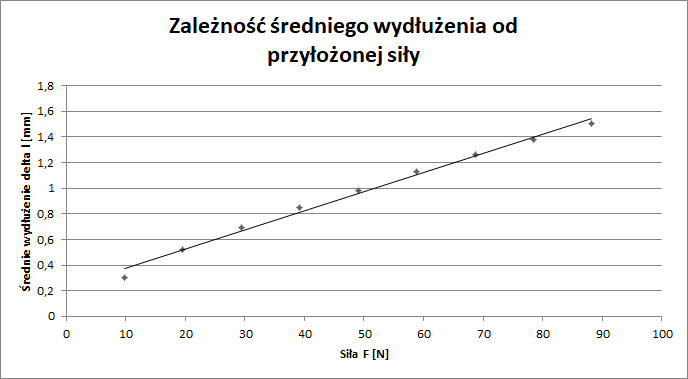
\includegraphics[scale=0.9]{W1}}
\end{figure}
\noindent
Ad. 5: Żaden z puntów nie odstaje w sposób znaczący znaczący od dopasowanej prostej.\\
Ad. 6: Uzyskane korzystając z programu Excel wartości $a = 0,01495 \hspace{5pt}u(a) = 0,00052$\\
Ad. 7: Podstawiając wartości do wzoru $E = \frac{4l}{\pi d^2 a}$ otrzymujemy $E = \frac{4*106*10^{-2}}{3,14 * (1,29*10^{-3})^2 * 0,01495} \approx 54,25[GPa]$\\
Ad. 8: Niepewność $\frac{u_c(E)}{E} = \sqrt{\left (\frac{-u(a)}{a} \right )^2 + \left (\frac{u(l)}{l} \right )^2 + \left (\frac{-2*u(d)}{d} \right )^2}$ $$u_c(E) = 54,25*\sqrt{\left (\frac{-0,00052}{0,01495} \right )^2 + \left (\frac{0,1}{106} \right )^2 + \left (\frac{-2*0,01}{1,29} \right )^2} = 2,07[GPa]$$ Niepewność rozszerzona $U(E) = 2*u_c(E) = 4,14[GPa]$\\
Ad. 9: Wartość tabelaryczną modułu Younga dla stali określa przedział 210-220 GPa co oznacza, że otrzymany wynik nie jest zgodny w granicach niepewności rozszerzonej.\vspace{15pt}\\
\noindent
\textit{Obliczenia dla drutu mosiężnego}

\noindent Ad. 1: Średnia wartość średnicy drutu wynosi $\frac{1,67 + 1,67 + 1,66}{3} \approx 1,67[mm]$ niepewność typu B jest równa najmniejszej podziałce i wynosi $1[mm]$.\\
Ad. 2: Wartości siły rozciągającej można znaleźć w tabeli.\\
Ad. 3: Średnie wartości wydłużenia można znaleźć w tabeli.\\
Ad. 4: 

\begin{figure}[h]
	\centering{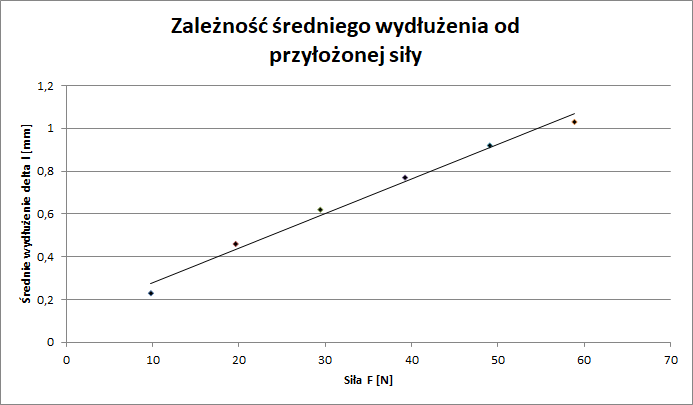
\includegraphics[scale=0.9]{W2}}
\end{figure}
\noindent
Ad. 5: Żaden z puntów nie odstaje w sposób znaczący znaczący od dopasowanej prostej.\\
Ad. 6: Uzyskane korzystając z programu Excel wartości $a = 0,01611 \hspace{5pt}u(a) = 0,00090$\\
Ad. 7: Podstawiając wartości do wzoru $E = \frac{4l}{\pi d^2 a}$ otrzymujemy $E = \frac{4*106,1*10^{-2}}{3,14 * (1,67*10^{-3})^2 * 0,01611} \approx 30,24[GPa]$\\
Ad. 8: Niepewność $\frac{u_c(E)}{E} = \sqrt{\left (\frac{-u(a)}{a} \right )^2 + \left (\frac{u(l)}{l} \right )^2 + \left (\frac{-2*u(d)}{d} \right )^2}$ $$u_c(E) = 30,24\sqrt{\left (\frac{-0,00090}{0,01611} \right )^2 + \left (\frac{0,1}{106,1} \right )^2 + \left (\frac{-2*0,01}{1,67} \right )^2} = 1,74[GPa]$$ Niepewność rozszerzona $U(E) = 2*u_c(E) = 3,48[GPa]$\\
Ad. 9: Wartość tabelaryczna modułu Younga dla mosiądzu wynosi 40 GPa co oznacza, że otrzymany wynik nie jest zgodny w granicach niepewności rozszerzonej.

	\section{Wnioski}

\end{document}
















\end{}